\documentclass[11pt]{elegantbook}
\definecolor{structurecolor}{RGB}{40,58,129}
\linespread{1.6}
\setlength{\footskip}{20pt}
\setlength{\parindent}{0pt}
\newcommand{\argmax}{\operatornamewithlimits{argmax}}
\newcommand{\argmin}{\operatornamewithlimits{argmin}}
\elegantnewtheorem{proof}{Proof}{}{Proof}
\elegantnewtheorem{claim}{Claim}{prostyle}{Claim}
\DeclareMathOperator{\col}{col}
\title{\textbf{STAT 426}}
\author{Wenxiao Yang}
\institute{Department of Mathematics, University of Illinois at Urbana-Champaign}
\date{}
\setcounter{tocdepth}{2}
\cover{cover.jpg}
\extrainfo{All models are wrong, but some are useful.}

% modify the color in the middle of titlepage
\definecolor{customcolor}{RGB}{32,178,170}
\colorlet{coverlinecolor}{customcolor}
\usepackage{cprotect}

\addbibresource[location=local]{reference.bib} % bib

\begin{document}

\maketitle
\frontmatter
\tableofcontents
\mainmatter

\chapter{Basic of Categorical Data}
\section{Variable Measurement}
\begin{center}\begin{figure}[htbp]
    \centering
    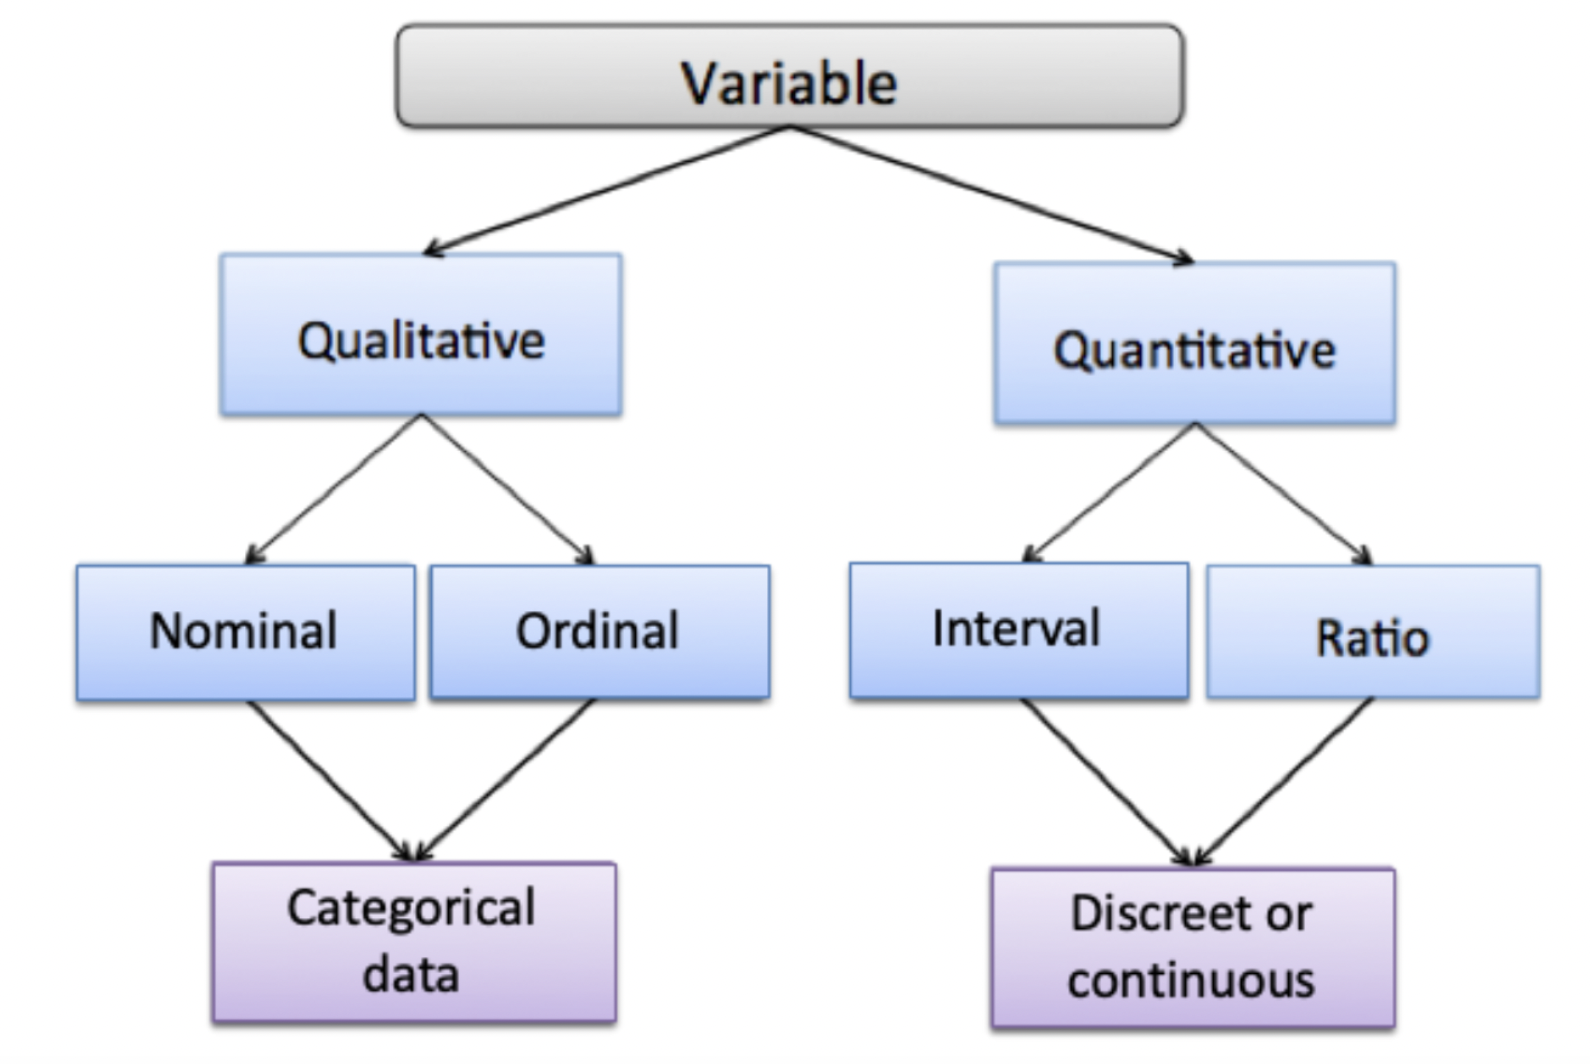
\includegraphics[scale=0.3]{p1.png}
    \caption{Variable Type}
    \label{}
\end{figure}\end{center}
\begin{enumerate}[a)]
    \item Nominal: Categories do not have a natural order. Ex. blood type, gender.
    \item Ordinal: Categories have a natural order. Ex. low/middle/high education level
    \item Interval: There is a numerical distance (difference between two different values is meaningful) between any two values.
    Ex. blood pressure level, 100 blood pressure doesn't mean the double degree of 50 pressure.
    \item Ratio: An interval variable where ratios are valid (presence of absolute zero, i.e. zero is meaningful). Ex. weight, 4g is double degree of 2g, distance run by an athlete.
\end{enumerate}
\subsection*{Levels of measurements}
A variable's level of measurement determines the statistical methods to be used for its analysis.
\begin{center}
    Variables hierarchy: Ratio $>$ Interval $>$ Ordinal $>$ Nominal
\end{center}
Statistical methods applied to variables at a lower level can be used with variables at a higher level, but the contrary is not true.

\section{Statistical Inference for Categorical Data}
Let $\beta$ a generic unknown parameter and $\hat{\beta}$ the parameter estimate.
\subsection{Maximum likelihood Estimation (MLE)}
$\hat{\beta}=\arg\max_{\beta} l(\beta,\vec{x})$ maximizes the likelihood function $l(\beta)$, $\hat{\beta}=\arg\max_{\beta}\ln l(\beta,\vec{x})$ also maximizes the logarithm of the likelihood function $L(\beta) = \log(l(\beta))$.

\begin{definition}[score function]
    The score function is $$u(\beta)=\frac{\partial L(\beta)}{\partial \beta}=\frac{\nabla l(\beta)}{l(\beta)}$$
\end{definition}

\begin{definition}[Fisher information]
    The (Fisher) information is $$\iota(\beta)=\mathbb{E}\left(u(\beta)u(\beta)^T\right)=-\mathbb{E}\left(\frac{\partial^2 L(\beta)}{\partial \beta^2}\right)=$$
\end{definition}

\begin{proposition}
    When the sample $x$ is made up of i.i.d. observations, the covariance matrix of the maximum likelihood estimator $\hat{\beta}$ is approximately equal to the inverse of the information matrix. $$\textnormal{Cov}(\hat{\beta})\approx(\iota(\beta))^{-1}$$
\end{proposition}
\begin{proof}
    Use $\vec{x}=x_1,...,x_n$ denote the $n$ i.i.d. observations. The log-likelihood of the sample is $$L(\beta,\vec{x})=\sum_{i=1}^n\log(l(\beta,x_i))$$
\end{proof}















\end{document}